% =============================================================================
%  Data engineering report — Project 3: e-commerce modern data stack (EN)
%  Build: latexmk -xelatex report-en.tex
% =============================================================================
\documentclass[11pt, a4paper, oneside, headings=normal, numbers=noenddot, DIV=12]{scrartcl}
\usepackage[english]{babel}
\usepackage{report-style}
\graphicspath{{../livraison/figures/en/}}
\sisetup{locale=UK, group-minimum-digits=4, group-separator={,}}

% --- Metadata ------------------------------------------------------------------
\newcommand{\ReportAuthor}{LUMU BAMANA MANASSE}
\newcommand{\ReportAuthorRole}{Data engineer}
\newcommand{\ReportShortTitle}{Brazilian e-commerce · Data engineering report}
\newcommand{\ReportFooter}{October 2026 · v1.0.0}
\newcommand{\ReportKicker}{Data engineering report · Project 3}
\newcommand{\ReportTitle}{Should we sell\\in Brazil?}
\newcommand{\ReportSubtitle}{A local modern data stack on 100,000 real orders:\\S3 data lake, dbt, DuckDB, Dagster, Docker and continuous integration}
\newcommand{\ReportMeta}{%
  \begin{tabularx}{\linewidth}{@{}>{\bfseries}l@{\hspace{1em}}Y@{}}
  Date & October 2026 \\
  Version & 1.0.0 (delivered and accepted) \\
  Client & Maison Caju (fictional company) · Engagement CAJ-2026-001 \\
  GitHub repository & \url{https://github.com/MediJr/olist-ecommerce-modern-data-stack} \\
  Language & English · \textit{version française disponible dans le dépôt}
  \end{tabularx}}
\newcommand{\ReportScenario}{Fictional scenario, real data: the client company and its contacts are invented to simulate a complete
  professional engagement. The data is the \emph{Brazilian E-Commerce Public Dataset by Olist}, published on Kaggle under the
  CC BY-NC-SA 4.0 licence (anonymised orders from 2016 to 2018). This project is not commissioned, endorsed or affiliated with Olist.}
\hypersetup{pdftitle={Should we sell in Brazil? Data engineering report}, pdfauthor={Lumu Bamana Manasse},
  pdfsubject={Local modern data stack: S3, dbt, DuckDB, Dagster, portfolio project}, pdflang={en-GB}}

\begin{document}
\sloppy
\MakeTitlePage

% =============================================================================
\section*{Document information}
\addcontentsline{toc}{section}{Document information}

\begin{tabularx}{\linewidth}{@{}>{\bfseries\sffamily}L{4.2cm}Y@{}}
\toprule
Project & Portfolio project 3: modern data stack (data lake, dbt, orchestration, CI) \\
Engagement & CAJ-2026-001: ``Should we launch on Brazilian marketplaces?'' \\
Client & Maison Caju, French home-textile brand (fictional), attention of Claire Dumont \\
Author & Lumu Bamana Manasse, data engineer \\
Period & October 2026 \\
Data & Olist, 99,441 orders placed from September 2016 to October 2018 \\
Status & \pill{good}{DELIVERED} \pill{good}{ACCEPTED} \\
Source code & \url{https://github.com/MediJr/olist-ecommerce-modern-data-stack} \\
\bottomrule
\end{tabularx}

\subsection*{Version history}
\begin{tabularx}{\linewidth}{@{}l l Y@{}}
\toprule
\textbf{Version} & \textbf{Date} & \textbf{Purpose} \\
\midrule
0.1 & 2026-10-23 & Scoping: brief, meeting minutes, statement of work \\
0.5 & 2026-10-23 & S3 lake, ingestion, dbt project, Dagster orchestration \\
0.9 & 2026-10-25 & Whole platform moved to Docker, continuous integration, dashboard \\
1.0.0 & 2026-10-25 & Acceptance on a fresh machine, final report (French and English) \\
\bottomrule
\end{tabularx}

\subsection*{Reading guide}
\begin{tabularx}{\linewidth}{@{}>{\bfseries}L{4.2cm}Y@{}}
Board & \hyperref[sec:summary]{1. Executive summary} and \hyperref[sec:results]{11. Results and recommendations} \\
Analyst (Hugo) & 6. dbt data model, 7. Quality and tests, 9. Operations \\
Engineer taking over & 4. Architecture, 5. Pipeline and orchestration, 13. Lessons learned, appendices \\
\end{tabularx}

\begingroup
\addtokomafont{sectionentry}{\color{primary}}
\setcounter{tocdepth}{2}
\tableofcontents
\endgroup
\clearpage

% =============================================================================
\section{Executive summary}\label{sec:summary}

\textbf{The need.} Maison Caju is considering selling its collections in Brazil through local marketplaces. Its board wants a quantified
market study, and its analyst must be able to \textbf{evolve the metrics alone, in SQL, without risk of regression}.
Data arrives as \textbf{monthly deliveries}.

\textbf{The solution.} A complete \textbf{modern data stack} that fits on a laptop and starts with a single command, \texttt{docker compose up}.
Each delivery is checked, then stored in an \textbf{S3 data lake} (Parquet, one partition per month). It is transformed by \textbf{dbt} on
\textbf{DuckDB} into a tested star schema, orchestrated by \textbf{Dagster} (sensors, partitions, replays), and served to a bilingual
dashboard. \textbf{Continuous integration} rebuilds and tests the whole chain on every change.

\kpirow{99,441}{real orders\\(2016-2018)}{27 / 27}{successful runs\\on a fresh machine}{18 min}{from zero to\\dashboard}{94 / 94}{dbt models\\and tests}
\kpirow{0}{duplicate\\on replay}{= source}{revenue reconciled\\to the cent}{14}{Python\\tests}{6}{documented\\decisions (ADR)}

\begin{keybox}[Key results for Maison Caju]
\begin{itemize}[leftmargin=1.2em]
  \item \textbf{Q1 · Where to sell:} BRL 13.5 M in revenue. Home categories weigh \textbf{19.8\%}, and bed \& bath
        (\emph{bed\_bath\_table}) is the 3\textsuperscript{rd} category. São Paulo, Rio and Minas Gerais make \textbf{63\%} of revenue.
  \item \textbf{Q2 · Loyalty:} only \textbf{3.0\%} of customers order twice. This market is won through acquisition.
  \item \textbf{Q3 · Delivery:} the rating drops from \textbf{4.3 to 2.1} from 4 days late. The carrier choice is strategic.
  \item \textbf{Q4 · Payment:} credit card 75.5\%, \emph{boleto} 19.9\%. Baskets triple with 7 to 10 instalments.
  \item \textbf{Q5 · Freight:} 13.8\% of item price in São Paulo, up to \textbf{28.5\%} in the North.
\end{itemize}
\end{keybox}

\textbf{What this project demonstrates in data engineering:} S3 data lake and partitioned Parquet, delivery contract, idempotent ingestion,
layered dbt modelling with data tests, unit tests, contract and source reconciliations, event-driven orchestration with Dagster,
concurrency management for a single-writer warehouse, full containerisation and continuous integration.

% =============================================================================
\section{Context and scoping}

\subsection{What the request implies technically}
\begin{table}[H]
\centering\small
\begin{tabularx}{\linewidth}{@{}L{5.4cm} Y@{}}
\toprule
\textbf{Client request} & \textbf{Technical consequence} \\
\midrule
``Hugo must evolve the metrics without breaking what works'' & Business logic in \textbf{versioned, tested SQL} (dbt), mandatory \textbf{continuous integration} \\
``A very detailed dataset'' (9 tables) & \textbf{Dimensional model}: explicit grain, star schema \\
``A dashboard for the board'' & It reads \textbf{pre-computed, tested} tables, never raw files \\
Monthly exports from the partner & \textbf{Partitions} per delivery, duplicate-free \textbf{replays}, an \textbf{orchestrator} \\
\bottomrule
\end{tabularx}
\caption{From request to technical requirements}
\end{table}

\subsection{Scoping decisions}
\begin{table}[H]
\centering\small
\begin{tabularx}{\linewidth}{@{}l L{3cm} Y@{}}
\toprule
\textbf{\#} & \textbf{Topic} & \textbf{Decision} \\
\midrule
D1 & Updates & One export per month; simulated by splitting the public dataset by purchase month \\
D2 & Revenue & Item price, excluding freight, orders neither cancelled nor unavailable. Defined \textbf{once}, in dbt \\
D3 & Repeat customer & Customer identified by \texttt{customer\_unique\_id}; repeat = at least two valid orders \\
D4 & Dashboard & Metabase, later replaced by Streamlit (ADR 004) \\
D5 & Maintenance & Every change goes through a pull request tested by continuous integration \\
D6 & Language & Tables and columns in English; documentation in French, report also in English \\
\bottomrule
\end{tabularx}
\caption{Decisions of the 2026-10-23 scoping meeting}
\end{table}

\subsection{Business questions}
\begin{table}[H]
\centering\small
\begin{tabularx}{\linewidth}{@{}l Y L{4.4cm}@{}}
\toprule
\textbf{\#} & \textbf{Question} & \textbf{Decision supported} \\
\midrule
Q1 & Which categories and states drive revenue, and how does it evolve? & Launch collections and regions \\
Q2 & What share of customers comes back? & Loyalty or acquisition \\
Q3 & Does late delivery hurt the rating? & Carrier choice \\
Q4 & How do customers pay? & Payment offer \\
Q5 & How much does freight weigh by state? & Logistics cost by region \\
\bottomrule
\end{tabularx}
\caption{The five questions}
\end{table}

% =============================================================================
\section{Sources and profiling}

\subsection{The dataset}
The \emph{Brazilian E-Commerce Public Dataset by Olist} describes about 100,000 anonymised orders placed on a Brazilian marketplace
between 2016 and 2018, in \textbf{9 linked CSV files}: orders, items, payments, reviews, customers, sellers, products, geolocation and
category translations. The client downloaded it from Kaggle (personal account required) into \texttt{data/source/}.

\subsection{What profiling revealed}
\begin{table}[H]
\centering\small
\begin{tabularx}{\linewidth}{@{}L{5.6cm} Y@{}}
\toprule
\textbf{Finding} & \textbf{Risk if ignored, and treatment} \\
\midrule
\texttt{customer\_id}: 99,441 values for 96,096 people (\texttt{customer\_unique\_id}) & It changes with every order: loyalty would look \textbf{zero}. Count on \texttt{customer\_unique\_id} \\
2,961 orders paid in several payments (up to 29); 9,803 orders with several items & An items × payments join \textbf{multiplies revenue}. Aggregate each table before joining \\
98,410 \texttt{review\_id} for 99,224 reviews & \texttt{review\_id} alone is not a key: composite key (\texttt{review\_id}, \texttt{order\_id}) \\
2 untranslated categories, 610 products without category & Empty labels in the dashboard: explicit, tested fallback (\texttt{unknown}) \\
775 orders without items; 8 ``delivered'' orders without delivery date & Explicitly excluded from revenue or lead times \\
1,000,163 GPS points for 19,015 zip prefixes, some outside Brazil & Median per prefix, after geographic filtering \\
November 2016: no orders; September-October 2018: 20 orders, almost all cancelled & An empty delivery is still a delivery; analyses on complete months (01/2017-08/2018) \\
\bottomrule
\end{tabularx}
\caption{Profiling: seven traps, seven treatments}
\end{table}

% =============================================================================
\section{Architecture}

\begin{figure}[H]
\centering
\resizebox{\linewidth}{!}{%
\begin{tikzpicture}[
  font=\sffamily\small, node distance=0.6cm and 0.75cm,
  src/.style={draw=rule, fill=panel, rounded corners=2pt, minimum width=2.4cm, minimum height=1.1cm, align=center},
  stage/.style={draw=primary, fill=primary, text=white, rounded corners=3pt, minimum width=2.2cm, minimum height=1.2cm, align=center, font=\sffamily\small\bfseries},
  store/.style={cylinder, shape border rotate=90, aspect=0.18, draw=accent, fill=accent!8, minimum width=2.3cm, minimum height=1.3cm, align=center},
  arr/.style={-{Stealth[length=2.6mm]}, thick, color=ink2}]
  \node[src] (p) {Partner\\\scriptsize CSV + \_SUCCESS};
  \node[stage, right=of p] (i) {INGESTION\\\scriptsize\mdseries contract};
  \node[store, right=of i] (b) {\scriptsize S3 lake · bronze\\\scriptsize Parquet / month};
  \node[stage, right=of b] (s) {STAGING\\\scriptsize\mdseries typing};
  \node[stage, right=of s] (m) {INTERM.\\\scriptsize\mdseries rules};
  \node[store, right=of m] (w) {\scriptsize DuckDB · marts\\\scriptsize star schema};
  \node[src, right=of w] (d) {Streamlit\\\scriptsize FR / EN};
  \node[src, above=0.9cm of b, fill=white, draw=primary] (dag) {\textbf{Dagster}\\\scriptsize sensors · partitions};
  \draw[arr] (p) -- (i); \draw[arr] (i) -- (b); \draw[arr] (b) -- (s); \draw[arr] (s) -- (m); \draw[arr] (m) -- (w); \draw[arr] (w) -- (d);
  \draw[arr, dashed] (dag) -| (i); \draw[arr, dashed] (dag) -| (m);
  \begin{scope}[on background layer]
    \node[draw=rule, dashed, rounded corners=6pt, fit=(s)(m)(w), inner sep=8pt, label={[font=\scriptsize\sffamily, text=ink2]below:dbt build (models + tests)}] {};
  \end{scope}
\end{tikzpicture}}
\caption{From delivery to dashboard}
\end{figure}

\begin{table}[H]
\centering\small
\begin{tabularx}{\linewidth}{@{}L{2.6cm} L{3.6cm} Y@{}}
\toprule
\textbf{Role} & \textbf{Choice} & \textbf{Why} \\
\midrule
Data lake & S3-compatible storage (SeaweedFS), Parquet & Same interface as Amazon S3 or Google Cloud Storage: only the location changes to move to the cloud \\
Warehouse & DuckDB & Columnar, reads Parquet on S3 directly, nothing to administer \\
Transformations & dbt 1.12 & Versioned, tested, documented SQL with lineage: maintainable by an analyst \\
Orchestration & Dagster 1.13 & Thinks in \emph{assets}; each dbt model becomes an asset and each test a check \\
Serving & Streamlit & Versioned, tested dashboard, read-only on the warehouse \\
Runtime & Docker Compose & Three services; single \texttt{python:3.13-slim} image, pinned versions \\
Quality & GitHub Actions & The whole chain rebuilt and tested on every pull request \\
\bottomrule
\end{tabularx}
\caption{Technical choices (ADR 001, 002, 004, 005)}
\end{table}

The lake is set by a single variable, \texttt{LAKE\_URI}: \texttt{s3://olist-lake} in operation, a plain folder in continuous integration.
\textbf{The code cannot tell the difference}, which is what makes it portable to the cloud.

% =============================================================================
\section{Pipeline and orchestration}

\subsection{The delivery contract}
The partner drops one folder per month and writes the \texttt{\_SUCCESS} file \textbf{last}: a folder without this marker is a delivery
in progress, never read. Before anything is written to the lake, each file must meet its contract:

\begin{itemize}[leftmargin=1.2em]
  \item an \textbf{identical header}: an added, renamed or moved column blocks ingestion (schema drift);
  \item \textbf{non-empty, unique keys};
  \item an \textbf{all-text} read with declared columns: an empty month (header only) reads like a full one.
\end{itemize}

\subsection{The bronze layer: idempotent by design}
Each table of a month becomes \textbf{a single Parquet file}, laid out with the Hive convention that DuckDB, Spark and BigQuery all read:

\begin{lstlisting}[language={}]
s3://olist-lake/bronze/orders/delivery_month=2017-01/orders.parquet
\end{lstlisting}

Replaying a month \textbf{replaces} that file: a duplicate is impossible. Two lineage columns are added: \texttt{\_source\_file} (original
file) and \texttt{\_ingested\_at} (time it entered the lake).

\subsection{Event-driven orchestration}
\begin{table}[H]
\centering\small
\begin{tabularx}{\linewidth}{@{}L{3.6cm} Y@{}}
\toprule
\textbf{Dagster mechanism} & \textbf{Role} \\
\midrule
Dynamic partitions & A \texttt{delivery\_month} partition is created when a delivery is \textbf{received}, rather than a calendar fixed in advance \\
\texttt{landing\_sensor} & Every 30 s: a new \textbf{or re-delivered} month (modified marker) triggers the \texttt{monthly\_delivery} job \\
Run key \texttt{month@timestamp} & A given version of a delivery is never processed twice \\
Concurrency limit & DuckDB accepts a single writer: \textbf{one run at a time} (\texttt{dagster.yaml}) \\
Bootstrap & The monthly sensor waits for reference data; reference data arriving alone is loaded without dbt \\
Maximum runtime & 15 minutes per run, monitored by the daemon: a hang no longer blocks the queue \\
\bottomrule
\end{tabularx}
\caption{Orchestration (ADR 006)}
\end{table}

% =============================================================================
\section{dbt data model}

\subsection{Three layers, three roles}
\begin{table}[H]
\centering\small
\begin{tabularx}{\linewidth}{@{}L{2.6cm} L{2.2cm} Y@{}}
\toprule
\textbf{Layer} & \textbf{Models} & \textbf{Role} \\
\midrule
Staging (views) & 9 & One model per source: rename, type (\texttt{decimal} for money, never \texttt{float}), keep the latest delivery. \textbf{No business rule} \\
Intermediate (views) & 2 & \texttt{int\_orders}: one row per order and \textbf{all} business rules, written once \\
Marts (tables) & 6 + 5 & Star schema, plus one reporting table per question \\
\bottomrule
\end{tabularx}
\caption{The 22 dbt models (ADR 003)}
\end{table}

\subsection{The star schema}
The main fact table, \texttt{fct\_order\_items}, has \textbf{the item sold as its grain}: the finest level that carries revenue. One can
always aggregate up (order, category, month), never drill down. It is surrounded by \texttt{dim\_customers} (real customer),
\texttt{dim\_products}, \texttt{dim\_sellers} and \texttt{dim\_date}. A second fact table, \texttt{fct\_orders}, carries order-level
measures: delivery, review, payment.

\subsection{The rule that prevents multiplying revenue}
An order with 2 items and 2 payments yields \textbf{4 rows} if raw tables are joined. \texttt{int\_orders} therefore aggregates each child
table \textbf{before} joining:

\begin{lstlisting}[language=DuckSQL]
with items as (
    select order_id, count(*) as item_count, sum(price) as items_value,
           sum(freight_value) as freight_value
    from {{ ref('stg_order_items') }} group by order_id
),
payments as (
    select order_id, sum(payment_value) as payment_value, count(*) as payment_count
    from {{ ref('stg_order_payments') }} group by order_id
)
select ... from {{ ref('stg_orders') }} o
left join items using (order_id) left join payments using (order_id)
\end{lstlisting}

This rule is locked by a \textbf{dbt unit test} (two items, two payments, expected amounts) and by a \textbf{reconciliation} with the source
(section~\ref{sec:quality}).

% =============================================================================
\section{Quality and tests}\label{sec:quality}

\begin{table}[H]
\centering\small
\begin{tabularx}{\linewidth}{@{}L{4.4cm} Y r@{}}
\toprule
\textbf{Type} & \textbf{What is checked} & \textbf{Count} \\
\midrule
dbt data tests & Uniqueness, not null, relationships, accepted values (statuses, ratings, 27 states) & 69 \\
dbt unit tests & Validity and delay; no amount multiplication; real-customer order rank & 3 \\
Reconciliations (singular tests) & Mart revenue = bronze total; payments = bronze total; full cohort at month 0 & 3 \\
Enforced contract & Columns and types of \texttt{fct\_order\_items} & 1 \\
Python tests (pytest) & Delivery splitting, contract, idempotency, empty month, dashboard & 14 \\
\bottomrule
\end{tabularx}
\caption{The safety nets}
\end{table}

\begin{keybox}[Reconciliation with the source]
The \texttt{assert\_revenue\_reconciles\_with\_source} test recomputes revenue \textbf{directly on the bronze layer}, without any dbt model,
and compares it to the dashboard's. Result: \textbf{BRL 13,494,400.74 on both sides}, to the cent. If a join loses or duplicates an
item, the totals diverge and the build fails.
\end{keybox}

\subsection{Continuous integration that bites}
For acceptance, a classic mistake was introduced on purpose: \textbf{adding freight to revenue}.

\begin{terminal}{dbt build · deliberate bug}
\begin{lstlisting}[style=terminal]
# 1. freight added: the column type changes
Compilation Error in model fct_order_items
  This model has an enforced contract that failed.

# 2. freight added, keeping the same type
94 of 94 FAIL 1 assert_revenue_reconciles_with_source ......... [FAIL 1]
Done. PASS=93 WARN=0 ERROR=1 SKIP=0 TOTAL=94          (exit code: 1)
\end{lstlisting}
\end{terminal}

The two nets complement each other: the \textbf{contract} protects the shape (columns, types), the \textbf{reconciliation} protects the
substance (amounts). In both cases dbt exits with an error, so the pull request would be rejected.

% =============================================================================
\section{Security and personal data}
\begin{itemize}[leftmargin=1.2em]
  \item Data \textbf{anonymised by the publisher}: hashed identifiers, no names or addresses; only city, state and zip prefix remain.
  \item Secrets (S3 keys) in \texttt{.env}, excluded from Git; the S3 identity file is generated when the container starts.
  \item Services exposed on \texttt{127.0.0.1} only; containers run as an \textbf{unprivileged user}.
  \item The dashboard mounts the warehouse \textbf{read-only}.
  \item CC BY-NC-SA 4.0 licence: the full archive is not redistributed; only an attributed 450-order sample is used by CI.
\end{itemize}

% =============================================================================
\section{Operations}
\begin{table}[H]
\centering\small
\begin{tabularx}{\linewidth}{@{}L{4.6cm} Y@{}}
\toprule
\textbf{Need} & \textbf{Command or tool} \\
\midrule
Start the platform & \texttt{docker compose up -d -{}-build} \\
Receive a delivery & Drop the month's folder into \texttt{data/landing/}: the sensor does the rest \\
Replay a corrected month & Re-deliver the folder (new \texttt{\_SUCCESS}) or re-run the partition in Dagster \\
Monitor runs & Dagster UI, \url{http://127.0.0.1:3000}: graph, partitions, checks, logs \\
Change a metric & Edit the dbt model, then \texttt{docker compose run -{}-rm dagster python -m olist\_pipeline.dbt\_cli build} \\
Run Python tests & \texttt{docker compose run -{}-rm dagster pytest} \\
\bottomrule
\end{tabularx}
\caption{Day-to-day operations}
\end{table}

% =============================================================================
\section{Acceptance}
Acceptance ran on a \textbf{simulated fresh machine}: Docker volumes deleted, empty landing zone. The 26 deliveries and the reference data
were dropped at once, then processed with no intervention: \textbf{27 successful runs out of 27, in 18 minutes}, with a median of 19 s of
processing per month.

\begin{table}[H]
\centering\small
\begin{tabularx}{\linewidth}{@{}l Y c@{}}
\toprule
\textbf{\#} & \textbf{Criterion} & \textbf{Result} \\
\midrule
C1 & Starts on a fresh machine by following the README & \ok \\
C2 & One month = one partition; processing a month does not reprocess the others & \ok \\
C3 & Replaying a month creates no duplicate (October 2016 re-delivered: 329 orders before and after) & \ok \\
C4 & Mart revenue equals the source total (BRL 13,494,400.74) & \ok \\
C5 & All dbt tests pass (94/94); every model is documented & \ok \\
C6 & CI fails when a test breaks (demonstration above) & \ok \\
C7 & The dashboard answers Q1-Q5 (5 tabs, 10 charts, FR/EN) & \ok \\
C8 & No secret or raw data in version control & \ok \\
\bottomrule
\end{tabularx}
\caption{Acceptance criteria: 8 out of 8}
\end{table}

% =============================================================================
\section{Results and recommendations}\label{sec:results}

\subsection*{Q1 · Where is revenue made?}
\begin{figure}[H]
\centering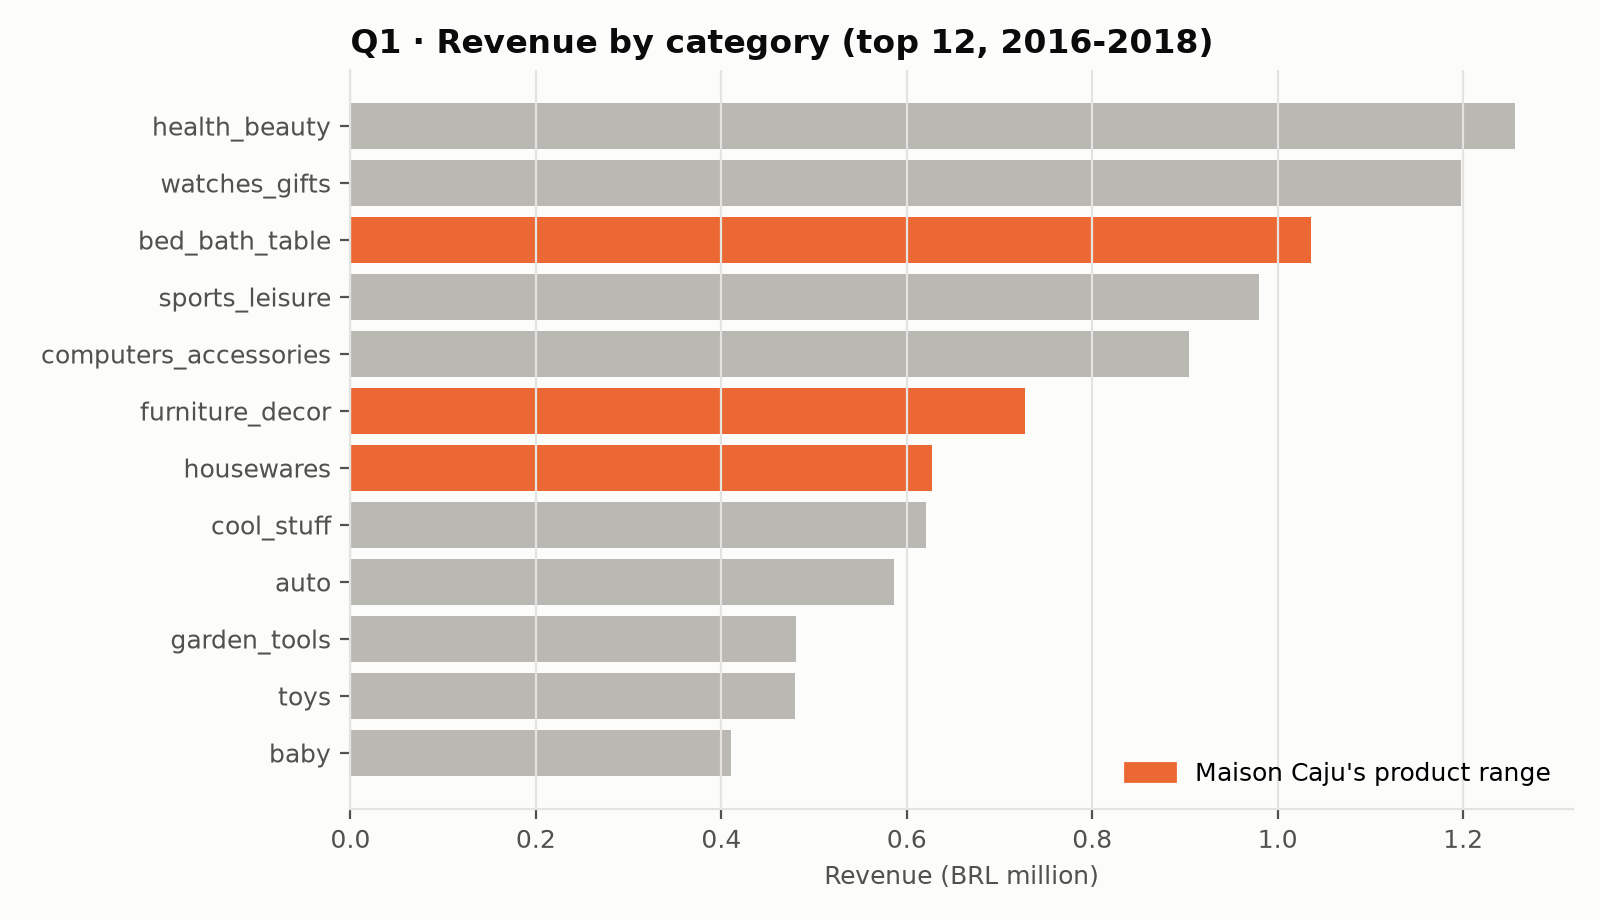
\includegraphics[width=0.86\linewidth]{q1_ca_par_categorie.png}
\end{figure}
Across 98,207 valid orders, revenue reaches \textbf{BRL 13.5 M} (excluding freight). Maison Caju's product range weighs \textbf{19.8\%},
and bed \& bath (\emph{bed\_bath\_table}, 7.7\%) is the market's 3\textsuperscript{rd} category.

\begin{figure}[H]
\centering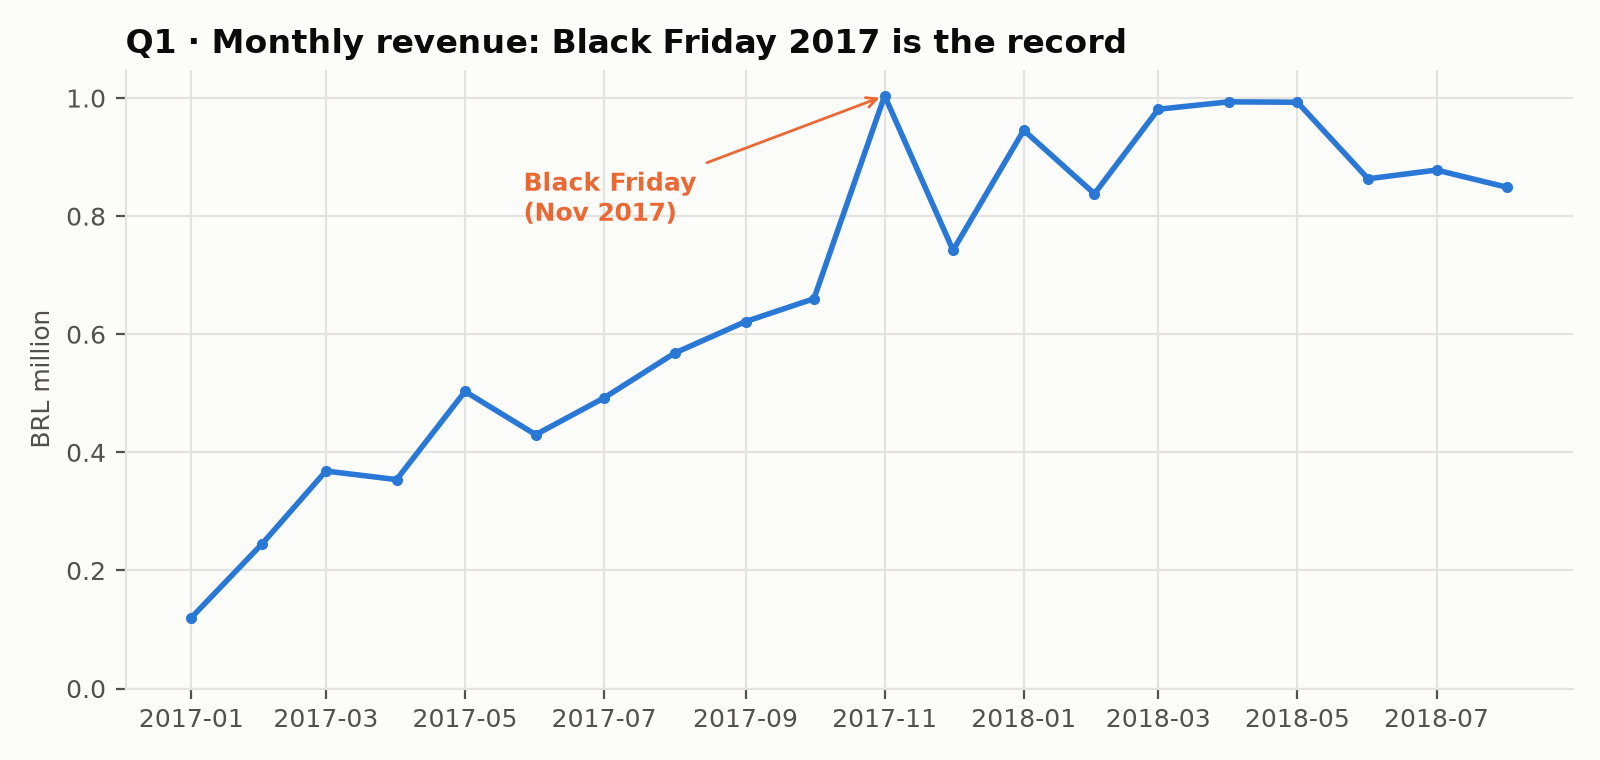
\includegraphics[width=0.86\linewidth]{q1b_ca_mensuel.png}
\end{figure}
The market grew strongly in 2017, then stabilised around BRL 0.9 M per month in 2018. \textbf{Black Friday 2017} beat October by
\textbf{52\%}.

\begin{figure}[H]
\centering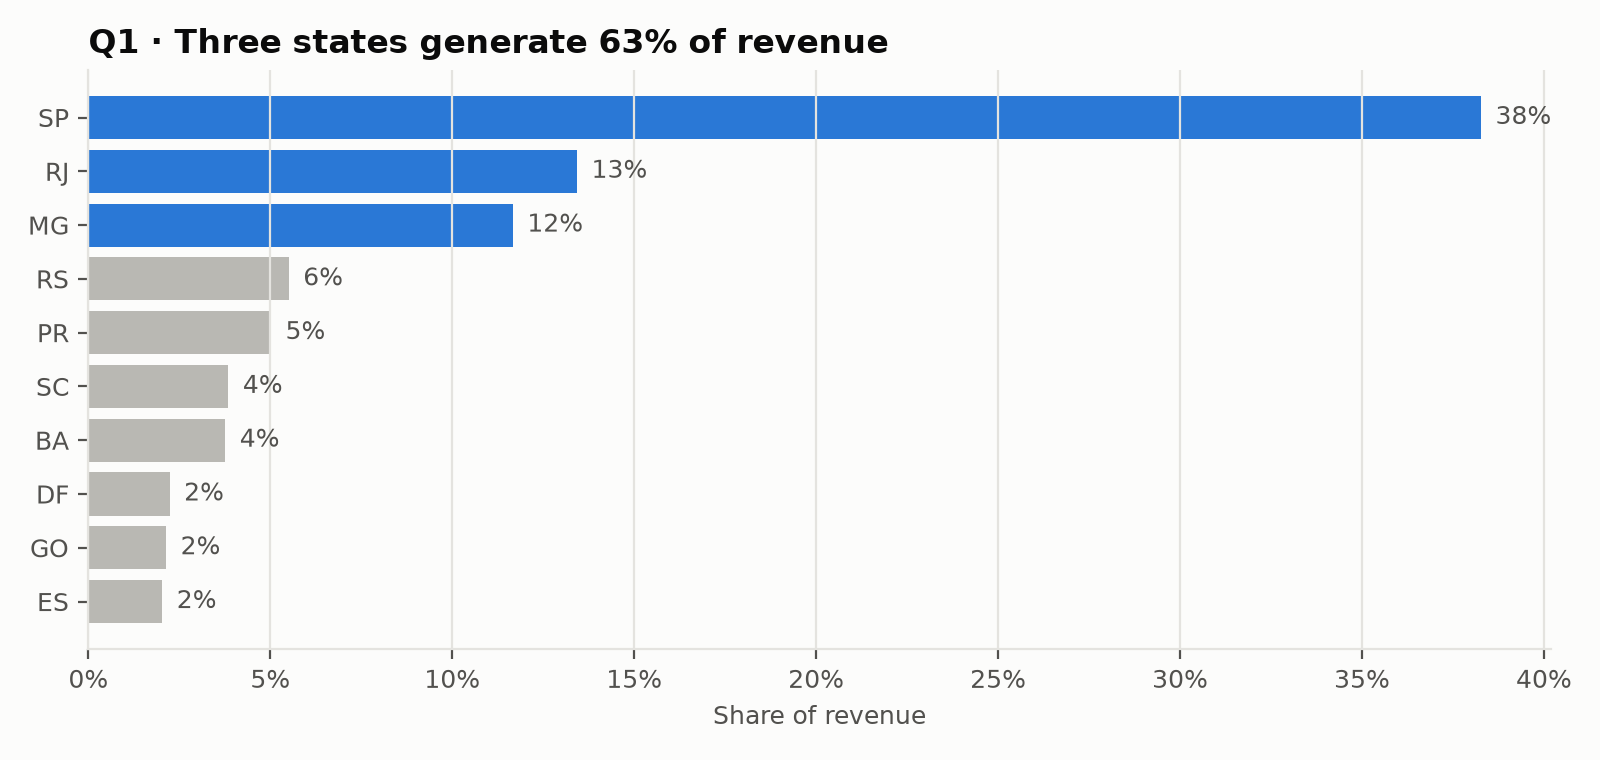
\includegraphics[width=0.86\linewidth]{q1c_ca_par_etat.png}
\end{figure}

\subsection*{Q2 · Do customers come back?}
\begin{figure}[H]
\centering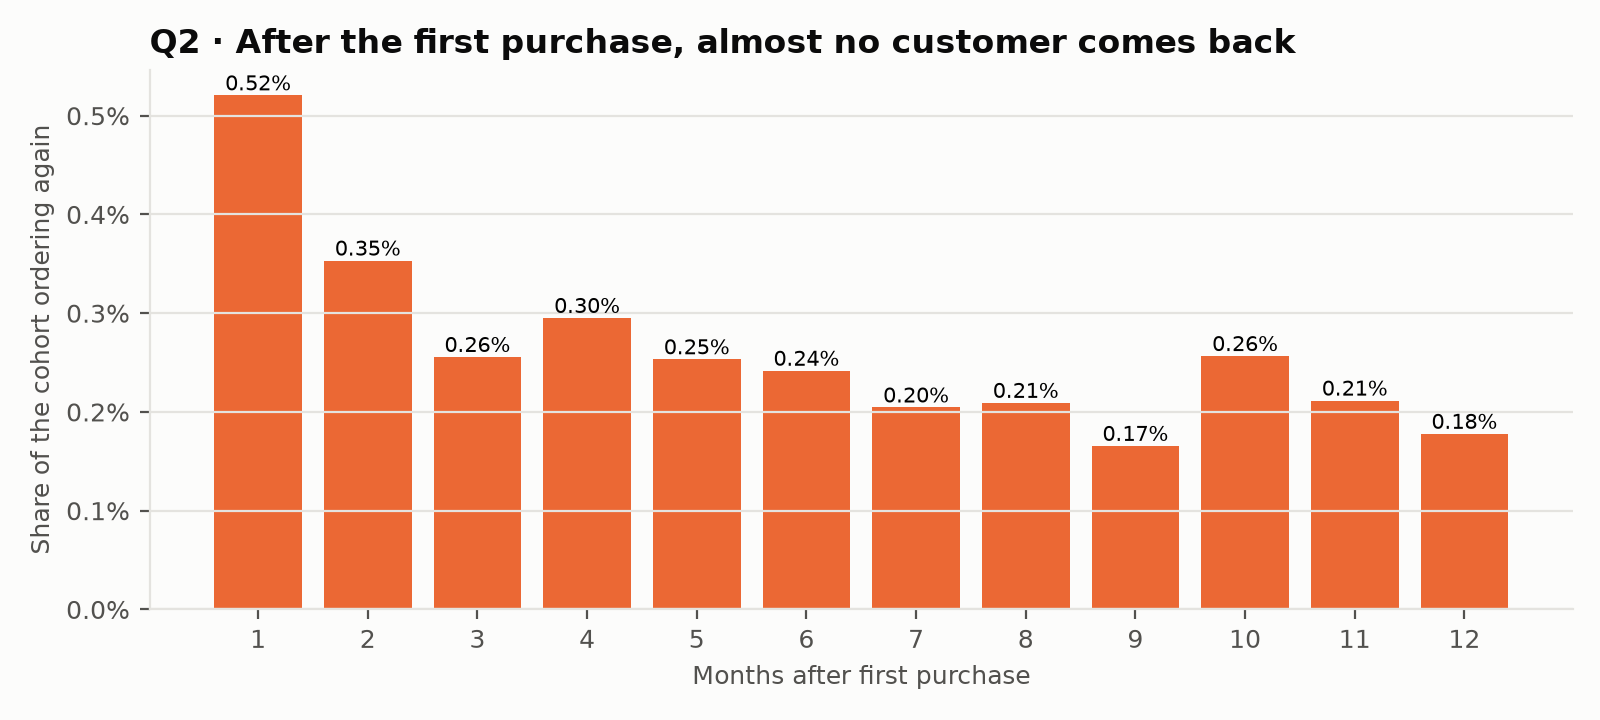
\includegraphics[width=0.86\linewidth]{q2_retention.png}
\end{figure}
Of 94,990 customers with a valid order, only \textbf{2,888 (3.0\%)} placed a second one, a median of 28 days later. One month after their
first purchase, barely \textbf{0.5\%} of 2017 customers order again.

\subsection*{Q3 · Does late delivery cost reviews?}
\begin{figure}[H]
\centering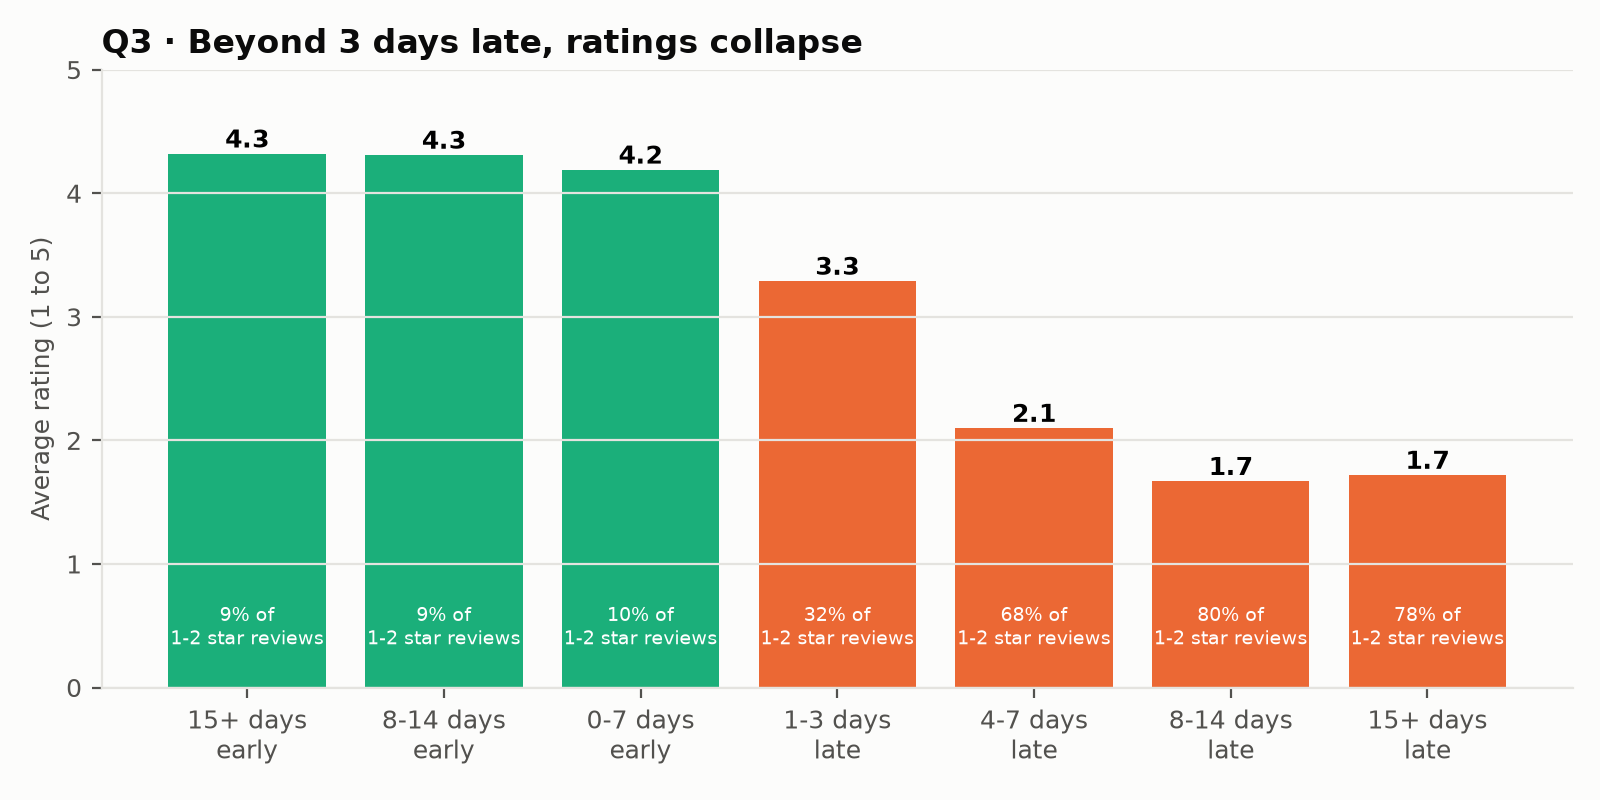
\includegraphics[width=0.86\linewidth]{q3_note_selon_retard.png}
\end{figure}
6.8\% of delivered orders arrive late. The average rating falls from \textbf{4.3} (on time or early) to \textbf{2.1} at 4 to 7 days late.
Beyond a week, \textbf{80\%} of reviews are 1 or 2 stars.

\subsection*{Q4 · How do customers pay?}
\begin{figure}[H]
\centering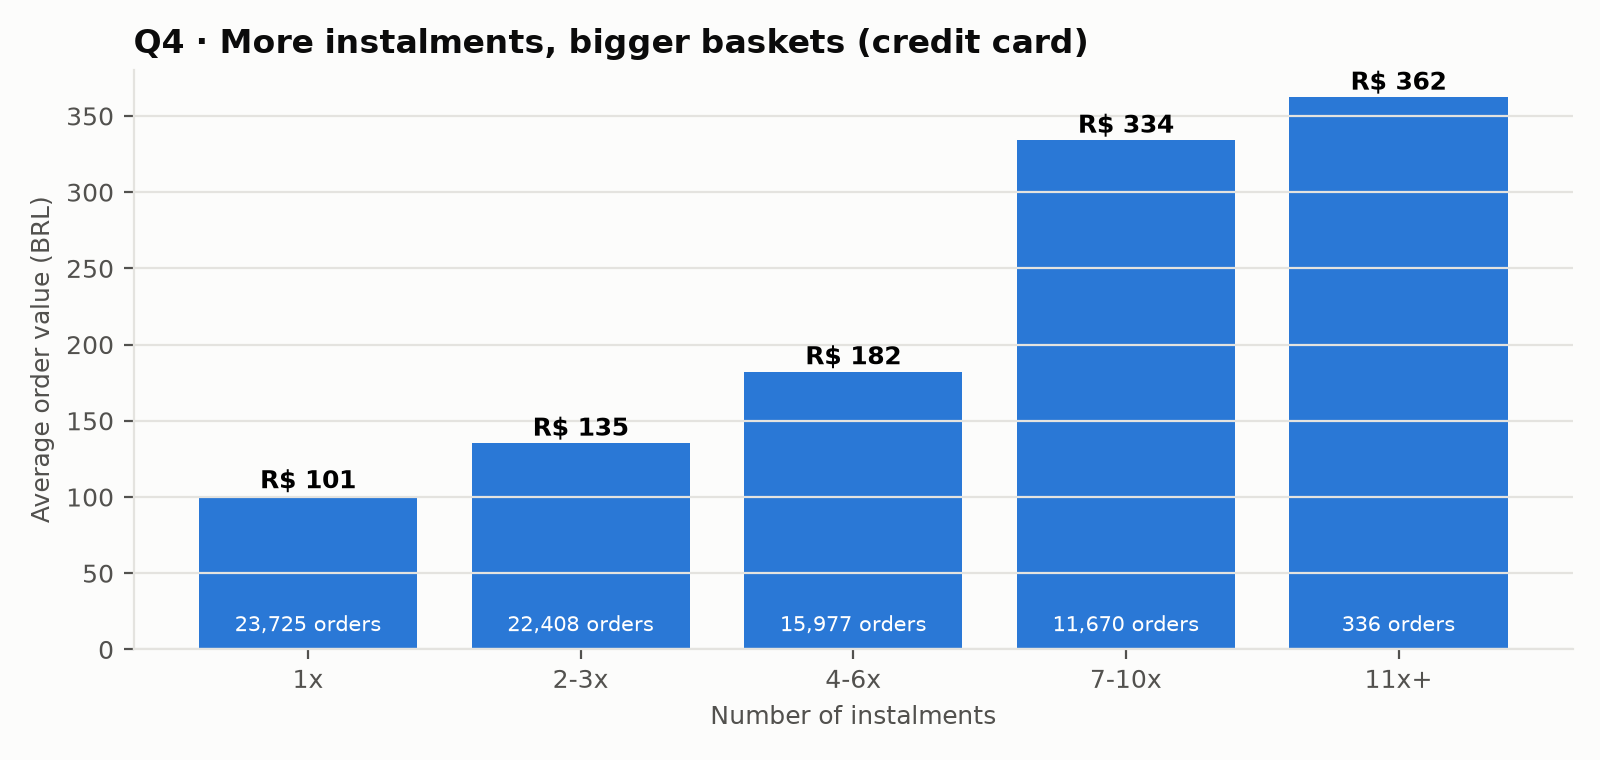
\includegraphics[width=0.86\linewidth]{q4_paiement_versements.png}
\end{figure}
Credit cards settle 75.5\% of orders, \emph{boleto} (a payment slip paid in cash or online) 19.9\%. With a card, the average basket rises
from \textbf{BRL 101} in one instalment to \textbf{BRL 334} in 7 to 10 instalments.

\subsection*{Q5 · How much does freight weigh?}
\begin{figure}[H]
\centering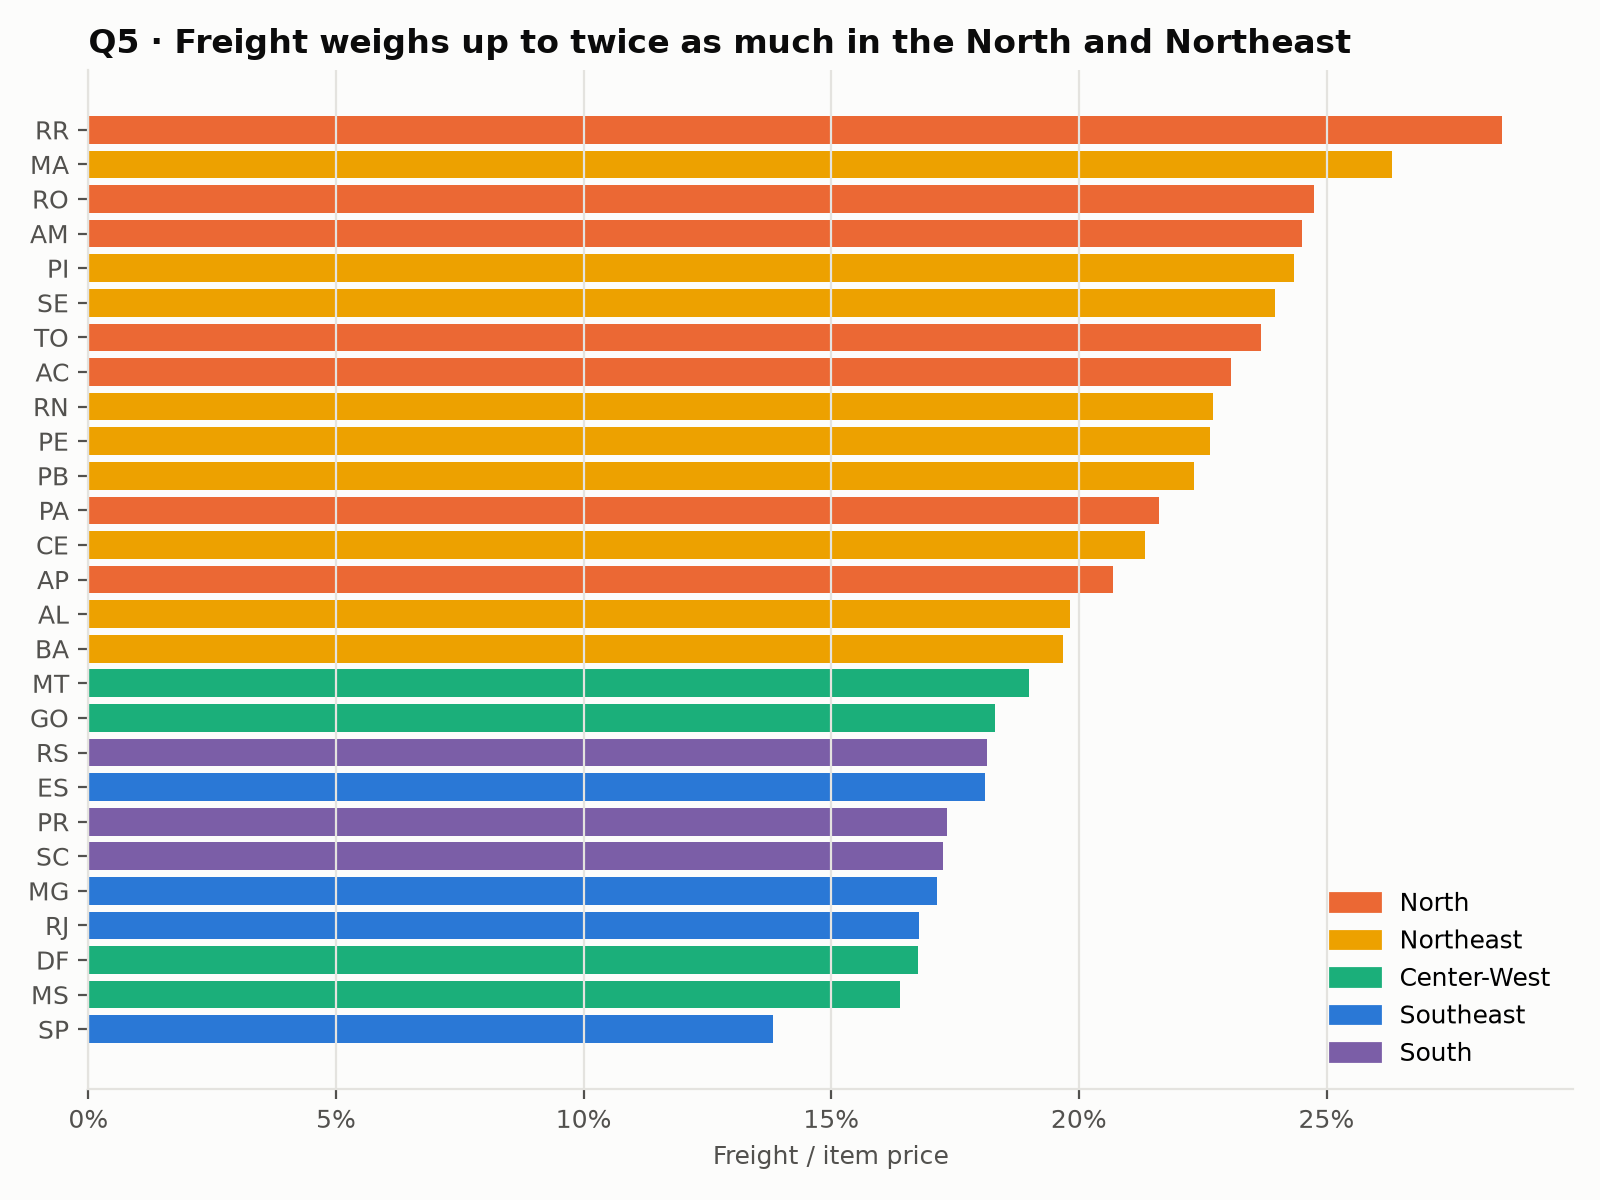
\includegraphics[width=0.78\linewidth]{q5_fret_par_etat.png}
\end{figure}
Freight is 13.8\% of item price in São Paulo (8.7 days average delivery), but \textbf{up to 28.5\%} in Roraima (29 days). The North and
Northeast combine high freight, long lead times and more frequent delays.

\begin{keybox}[Recommendations to the board]
\begin{enumerate}[leftmargin=1.4em]
  \item \textbf{Launch with bed \& bath and home decor}, already the market's 3\textsuperscript{rd} and 6\textsuperscript{th} categories.
  \item \textbf{Start with the Southeast} (São Paulo, Rio, Minas Gerais): 63\% of revenue, the lowest freight and the shortest lead times.
        The North and Northeast come next, with a dedicated freight policy.
  \item \textbf{Invest in acquisition rather than loyalty}: 97\% of customers buy only once. Prepare for Black Friday.
  \item \textbf{Choose the carrier on punctuality} and promise realistic lead times: a few days late halves the rating.
  \item \textbf{Offer instalments and \emph{boleto}}: the average basket triples with instalments.
\end{enumerate}
\end{keybox}

% =============================================================================
\section{Limitations}
\begin{itemize}[leftmargin=1.2em]
  \item The data covers 2016-2018: it describes the market's \textbf{structure}, not its current state, and comes from a single marketplace.
  \item Revenue is that of all the marketplace's sellers, not of a brand comparable to Maison Caju.
  \item The warehouse is rebuilt at each delivery (about 20 s): right for this volume, not for hundreds of millions of rows.
  \item \texttt{dagster dev} runs server and daemon in one container with SQLite history: right for a laptop, not for production.
\end{itemize}

% =============================================================================
\section{Lessons learned}
\begin{table}[H]
\centering\small
\begin{tabularx}{\linewidth}{@{}L{3.9cm} Y@{}}
\toprule
\textbf{Incident} & \textbf{Lesson} \\
\midrule
MinIO image no longer published & An open-source component can change its distribution model. Thanks to the S3 standard, SeaweedFS replaced it \textbf{without changing a line of code} (ADR 002) \\
dbt run before the first order & A platform's start-up order is a dependency like any other: it must be \textbf{explicit} (bootstrap, ADR 006) \\
\texttt{dagster-dbt} requires Python < 3.14 & Check the compatibility of the \textbf{whole} chain before choosing a version \\
Smart App Control blocks unsigned DLLs; a run hung for 83 min and blocked the queue & A single-run queue needs a \textbf{maximum runtime}. Containerisation makes the platform independent of the machine (ADR 005) \\
Dashboard test fails in CI & The default period was hard-coded: a test on different data reveals \textbf{hidden assumptions} \\
Delivery simulation took 3 min 30 & Filtering a table 26 times costs more than a single group-by: 26 s after the fix \\
\bottomrule
\end{tabularx}
\caption{What this project taught}
\end{table}

% =============================================================================
\section{Roadmap}
\begin{enumerate}[leftmargin=1.4em]
  \item \textbf{Move to the cloud} (project 6): lake on Google Cloud Storage, BigQuery warehouse, same dbt structure, infrastructure as code.
  \item \textbf{Incremental dbt models} if volume or frequency grows.
  \item \textbf{Production Dagster}: separate server, daemon and PostgreSQL storage; failure alerts.
  \item \textbf{Source freshness}: alert if no delivery arrives within 35 days (\texttt{dbt source freshness}, already configured).
  \item \textbf{Review analysis} (Portuguese text) to understand the causes of dissatisfaction.
\end{enumerate}

% =============================================================================
\clearpage
\appendix
\section{Repository structure}
\begin{lstlisting}[language={}]
src/olist_pipeline/   config, landing, bronze, definitions (Dagster), dbt_cli, report
dbt/models/           staging (9) · intermediate (2) · marts/core (6) · marts/reporting (5)
dbt/tests/            3 reconciliations with the source
dashboard/app.py      Streamlit dashboard (FR/EN)
tests/                pytest + CI sample (450 real orders)
dagster_home/         Dagster configuration (concurrency, run monitoring)
docs/                 engagement, ADRs, work log, data dictionary, reports, acceptance
Dockerfile · docker-compose.yml · .github/workflows/ci.yml
\end{lstlisting}

\section{Continuous integration steps}
\begin{enumerate}[leftmargin=1.4em]
  \item Code style (\texttt{ruff}) and Python tests (\texttt{pytest}).
  \item Simulated deliveries from the sample, then ingestion into a local lake (folder).
  \item \texttt{dbt build}: 22 models, 69 data tests, 3 unit tests.
  \item Dagster definitions validation, dashboard smoke test.
  \item Docker image build.
\end{enumerate}

\end{document}
